\documentclass[11pt,twocolumn]{article}
\usepackage[margin=0.72in]{geometry}
\usepackage{amsmath,amssymb,amsthm}
\usepackage{booktabs}
\usepackage{graphicx}
\usepackage{hyperref}
\usepackage{xcolor}
\usepackage{enumitem}

\hypersetup{
  colorlinks=true,
  linkcolor=blue!60!black,
  citecolor=green!45!black,
  urlcolor=blue!65!black
}

\newtheorem{proposition}{Proposition}
\newtheorem{definition}{Definition}

\newcommand{\ZZ}{\mathbb{Z}}
\newcommand{\QQ}{\mathbb{Q}}
\newcommand{\NN}{\mathbb{N}}

\title{\textbf{Machine-Checked Exact-Rational Koszul Complex Exactness, Max-Degree Filtration, and Multicolor Permutation Wordle Dimension-Count Certificates}}
\author{Lluis Eriksson\thanks{Independent researcher; manuscript prepared with transparent AI assistance via Google Antigravity. Source code, Lean~4 proofs, and exact certificates: \url{https://github.com/lluiseriksson/koszul-wordle-certificates}.}}
\date{November 25, 2026}

\begin{document}
\maketitle

\begin{abstract}
Lawren Smithline (\texttt{arXiv:2611.33113}, November 24, 2026) resolved Kutin and Smithline's Conjecture~4.5 on Multicolor Permutation Wordle by proving that the Koszul complex $K(N, M, b)$ of the ideals $J(M, N) = \bigl(\prod_{i=1}^N (x_i^{s_k} - v_k^{s_k}) : 1 \le k \le M\bigr)$ is exact at every \emph{gap-free} multidegree~$b$ (Theorem~5.1), yielding exact quotient dimensions $\dim R_n(d)/(J_n \cap R_n(d))$ matching the generating function $A_n(u)\prod_{k=1}^n(1+\dots+u^{s_k-1})$ (Theorem~6.1) and proving dominance of \textsc{CircularShift} (Theorem~1.1), while Appendix~A Remark~A.1 demonstrates that dropping gap-freeness breaks strictness. We present a machine-checked, zero-floating-point formalization and exact-$\QQ$ certificate auditor for the algebraic, homological, and rank-theoretic core of these results. First, an 18-theorem zero-dependency Lean~4 kernel (\texttt{KoszulWordle.lean}, Lean~4.35.0; 0~\texttt{sorry}, 0~warnings, 0~\texttt{Classical.choice}, 4 zero-axiom theorems) formalizes grade-2/3 Koszul $\delta^2=0$, filtration preservation, inductive Euler-characteristic telescoping on arbitrary finite exact chains, recursive Eulerian tables, both Smithline p.~19 dimension examples, inductive saturation degree $\sum s_k - 1$, uniform $|V(J_n)| = n!\,s^n$, and both Remark~A.1 non-gap-free counterexample identities and parity obstruction. Second, \texttt{KOSZUL-WORDLE-CERT-1.0} audits four exact-$\QQ$ modes—explicit Koszul differential matrices ($\delta^2=0$ and exactness at every $h\ge 1$), Theorem~6.1 generating functions, Farkas dual proofs $w^T\delta_1=0, w^TZ\neq 0$ of Remark~A.1 strictness failure, and rational evaluation ranks on $V(J_n) \subset \QQ^n$ up to 48 points—replaying 16 canonical certificates in $0.050$--$66.09\,\mathrm{ms}$ and rejecting 57/57 live adversarial forgeries.
\end{abstract}

\section{Introduction}
In Permutation Wordle~\cite{kutin2024wordle} and its multicolor generalization, a polynomial-method upper bound on the number of colored permutations solvable within $d+1$ rounds reduces to computing the dimension of the max-degree-filtered quotient $R_n(d) / (J_n \cap R_n(d))$ of $R_n = \mathbb{C}[x_1,\dots,x_n]$ modulo $J_n = (Q_1,\dots,Q_n)$, where $Q_k = \prod_{i=1}^n (x_i^{s_k} - v_k^{s_k})$~\cite{smithline2026koszul}. For $s_k = 1$, Garsia--Stanton descent monomials~\cite{garsia1984stanley} yield cumulative Eulerian numbers $\sum_{r \le d} A(n,r)$; for heterogeneous color counts $(s_1,\dots,s_n)$, Smithline~\cite{smithline2026koszul} deploys the filtered Koszul complex $K(N, M, b)$~\cite{eisenbud1995commutative}, proving exactness at every gap-free multidegree~$b$ (Theorem~5.1) via a two-axis induction (mapping cone in~$M$, multidegree reduction in~$N$), resolving Conjecture~4.5 (Theorem~6.1).

Because every Koszul differential $\delta_h : F_h^b(N, M) \to F_{h-1}^b(N, M)$, every Remark~A.1 counterexample ($N=M=2$, $b=(0,2)$ and $b=(2,4)$), and every evaluation matrix on the rational zero set $V(J_n) \subset \QQ^n$ (when $s_k \in \{1,2\}$) has exact rational entries, exact Gaussian elimination over~$\QQ$ eliminates floating-point rank instability completely and certifies homological exactness and strictness failures bit-for-bit.

\paragraph{Contributions.}
We formally verify and audit the finite homological, Euler-characteristic, counterexample, and evaluation-rank core of~\cite{smithline2026koszul} (explicitly scoping our Lean~4 proofs away from the general-parameter mapping-cone induction Theorem~5.1 and the game-theoretic feasible-history construction of Theorem~1.1):
\begin{enumerate}[leftmargin=*,nosep]
  \item \textbf{Zero-dependency Lean~4 kernel (\S\ref{sec:lean}):} 18 constructive theorems in \texttt{KoszulWordle.lean} (Lean~4.35.0~\cite{demoura2021lean4}), 0~\texttt{sorry}, 0~warnings, 0~\texttt{Classical.choice}, 4 zero-axiom theorems.
  \item \textbf{Exact-$\QQ$ homological \& dual verifier (\S\ref{sec:certifier}):} \texttt{KOSZUL-WORDLE-CERT-1.0}, auditing filtered Koszul differential matrices, Theorem~6.1 generating functions, Farkas dual strictness-failure certificates, and $V(J_n)$ evaluation ranks with zero floats.
  \item \textbf{Empirical atlas, strictness-defect map, \& red-team audit (\S\ref{sec:results}):} 16 canonical certificates replayed in $0.050$--$66.09\,\mathrm{ms}$, exhaustive 16-point gap-free defect grid, $V(J_3)$ rank sweeps, and 57/57 rejected adversarial forgeries.
\end{enumerate}

\section{Filtered Koszul Complexes and Strictness}\label{sec:prelim}
For $s_1,\dots,s_M \in \ZZ_{>0}$ and distinct $v_1,\dots,v_M \in \QQ_{>0}$ with $c_k = v_k^{s_k}$, let $Q_k = \prod_{i=1}^N (x_i^{s_k} - c_k)$. On $\bigwedge^h R_N^M$ with basis $e(T)$ ($|T|=h$, $\deg T = \sum_{k\in T} s_k$), the multidegree filtration $F_h^b(N,M) = \{Z : \deg_j Z(T) + \deg T \le b_j\;\forall j,T\}$ is preserved by $\delta e(T) = \sum_{k\in T} \mathrm{sign}(T,k) Q_k e(T\setminus\{k\})$. Whenever $K(N,M,b)$ is exact at all $h \ge 1$ (guaranteed by Theorem~5.1 when $b$ is \emph{gap-free}, i.e., its distinct entries form consecutive integers), Euler-characteristic telescoping gives
\begin{equation}
\begin{aligned}
  \dim R_N(b) - \mathrm{rank}\,\delta_1 &= \\
  \sum_{T \subseteq [M]} (-1)^{|T|} &\prod_{j=1}^N \max(0,\, b_j + 1 - \deg T),
\end{aligned}
  \label{eq:euler}
\end{equation}
which at $N=M=n, b=d\mathbf{1}_n$ matches the cumulative coefficients of $A_n(u)\prod_{k=1}^n (1+u+\dots+u^{s_k-1})$ and saturates at $n!\prod s_k$ at $d_{\max} = \sum s_k - 1$ (Theorem~6.1). Conversely, at non-gap-free multidegrees (Appendix~A Remark~A.1), $Z = (x_2 - c_2)Q_1 - (x_2 - c_1)Q_2 \in J(2,2) \cap R_2(0,2)$ lies outside $\mathrm{im}(\delta_1|_{F_1^{(0,2)}})$, certified cleanly by a rational Farkas dual functional $w \in \QQ^{\dim R_N(b)}$ with
\begin{equation}
  w^T \delta_1 = 0 \qquad \text{and} \qquad w^T Z \neq 0.
  \label{eq:farkas}
\end{equation}

\section{Zero-Dependency Lean 4 Kernel}\label{sec:lean}
We formalize 18 constructive theorems in \texttt{lean/KoszulWordle.lean} (Lean~4.35.0, zero external libraries), audited via \texttt{lean/AuditAxioms.lean} with 0~warnings, 0~\texttt{sorry}, 0~\texttt{Classical.choice}, and 0~\texttt{Lean.ofReduceBool} (Table~\ref{tab:lean}).

\begin{proposition}[Constructive Koszul \& Wordle Kernel]\label{prop:lean}
\leavevmode
\begin{enumerate}[leftmargin=*,nosep]
  \item \emph{Koszul differential \& inductive Euler characteristic:} Theorems~1--7 certify grade-2/3 $\delta^2 = 0$, filtration preservation $\delta(F_h^b) \subseteq F_{h-1}^b$, 2- and 3-step exactness identities, general inductive telescoping \texttt{koszul\_\allowbreak exactness\_\allowbreak euler\_\allowbreak char\_\allowbreak list} on arbitrary finite exact chains, and negative-coordinate box collapse.
  \item \emph{Eulerian tables \& Multicolor Wordle counts:} Theorems~8--12 and~18 prove recursive Eulerian numbers $A(n,r)$ ($n=1..4$), both Smithline p.~19 examples ($n=3, s=(1,1,1)$ and $n=2, s=(3,2)$), inductive saturation degree $(n-1)+\sum(s_k-1) = \sum s_k - 1$, uniform $|V(J_n)| = n!\,s^n$, and the Section~6.1 feasible-history bound.
  \item \emph{Remark~A.1 counterexamples \& gap-freeness:} Theorems~13--17 prove both exact algebraic identities for $s=(1,1), b=(0,2)$ and $s=(2,2), b=(2,4)$, the odd-vs.-even parity obstruction ($Z(-x)= -Z(x) \land E(-x)=E(x) \land Z=E \implies Z=0$), uniform spread~$0$, and shift invariance of pairwise differences.
\end{enumerate}
\end{proposition}

\begin{table}[t]
\centering
\caption{Complete 18-theorem Lean~4.35.0 kernel in \texttt{KoszulWordle.lean} (0~\texttt{sorry}, 0~warnings, 0~\texttt{Classical.choice}).}
\label{tab:lean}
\resizebox{\columnwidth}{!}{%
\begin{tabular}{@{}rll@{}}
\toprule
\# & Lean~4 Theorem Identifier & Axiom Footprint \\
\midrule
1 & \texttt{koszul\_d2\_square\_zero} & \texttt{[propext, Quot.sound]} \\
2 & \texttt{koszul\_d3\_square\_zero} & \texttt{[propext, Quot.sound]} \\
3 & \texttt{koszul\_filtration\_preserved\_by\_diff} & \texttt{[propext, Quot.sound]} \\
4 & \texttt{koszul\_exactness\_euler\_char\_2} & \texttt{[propext, Quot.sound]} \\
5 & \texttt{koszul\_exactness\_euler\_char\_3} & \texttt{[propext, Quot.sound]} \\
6 & \texttt{koszul\_exactness\_euler\_char\_list} & \texttt{[propext, Quot.sound]} \\
7 & \texttt{filtered\_rn\_dim\_zero\_if\_neg} & \texttt{[propext]} \\
8 & \texttt{eulerian\_number\_table\_exact} & \texttt{none} \\
9 & \texttt{worpitzky\_cumul\_n3\_exact} & \texttt{none} \\
10 & \texttt{multicolor\_dim\_n2\_s32\_exact} & \texttt{none} \\
11 & \texttt{saturation\_degree\_formula} & \texttt{[propext, Quot.sound]} \\
12 & \texttt{zero\_set\_cardinality\_uniform} & \texttt{none} \\
13 & \texttt{remark\_A1\_s11\_counterexample\_identity} & \texttt{[propext, Quot.sound]} \\
14 & \texttt{remark\_A1\_s22\_counterexample\_identity} & \texttt{[propext, Quot.sound]} \\
15 & \texttt{remark\_A1\_even\_vs\_odd\_obstruction} & \texttt{[propext, Quot.sound]} \\
16 & \texttt{gap\_free\_uniform\_multidegree} & \texttt{[propext, Quot.sound]} \\
17 & \texttt{gap\_free\_shifted\_invariant} & \texttt{[propext, Quot.sound]} \\
18 & \texttt{feasible\_history\_dim\_bound} & \texttt{[propext, Quot.sound]} \\
\bottomrule
\end{tabular}}
\end{table}

\section{Exact-Rational Certificate Architecture}\label{sec:certifier}
The pure-stdlib verifier \texttt{src/koszul\_certifier.py} audits \texttt{KOSZUL-WORDLE-CERT-1.0} certificates with zero floating-point arithmetic and strict JSON AST typing (rejecting \texttt{float}, \texttt{bool}, \texttt{Decimal}, \texttt{complex}, tuples, non-string keys, unreduced fractions, denominator-1 strings, and \texttt{"-0"}) across four exact modes:

\begin{definition}[Four \texttt{KOSZUL-WORDLE-CERT-1.0} Modes]\label{def:modes}
\leavevmode
\begin{enumerate}[leftmargin=*,nosep]
  \item \textbf{Mode~1} (\texttt{\small koszul\_\allowbreak filtered\_\allowbreak exactness\_\allowbreak exact}): Audits gap-free $b \in \ZZ^N$, constructs exact rational matrices $\delta_h$ ($h=1..M$), verifies $\delta_h \delta_{h+1} = 0$, verifies exactness $\mathrm{rank}\,\delta_h + \mathrm{rank}\,\delta_{h+1} = \dim F_h^b$ at every $h \ge 1$, and matches $\dim R_N(b) - \mathrm{rank}\,\delta_1$ to Eq.~\eqref{eq:euler}.
  \item \textbf{Mode~2} (\texttt{\small multicolor\_\allowbreak wordle\_\allowbreak dim\_\allowbreak count\_\allowbreak exact}): Audits $W_s(u) = A_n(u)\prod(1+\dots+u^{s_k-1})$, saturation degree $\sum s_k - 1$, total $n!\prod s_k$, and exact agreement with Eq.~\eqref{eq:euler} at every $d \in [0, d_{\max}]$.
  \item \textbf{Mode~3} (\texttt{\small gap\_\allowbreak free\_\allowbreak strictness\_\allowbreak failure\_\allowbreak exact}): Audits a non-gap-free $b$, nonzero $Z = \sum_k A_k Q_k \in J(M,N) \cap R_N(b)$, and exact Farkas dual vector $w$ satisfying~\eqref{eq:farkas} ($Z \notin \mathrm{im}\,\delta_1$).
  \item \textbf{Mode~4} (\texttt{\small zero\_\allowbreak set\_\allowbreak eval\_\allowbreak rank\_\allowbreak exact}): For $s_k \in \{1,2\}$, constructs the exact rational zero set $V(J_n) \subset \QQ^n$ of size $n!\prod s_k$ and verifies by exact rational Gaussian elimination that $\mathrm{rank}\,E_{V(J_n)}(R_n(d))$ equals Eq.~\eqref{eq:euler}.
\end{enumerate}
\end{definition}

\section{Empirical Atlas and Red-Team Verification}\label{sec:results}
All 16 canonical certificates and four experiment logs are generated deterministically by \texttt{scripts/run\_all\_experiments.py} and audited end-to-end by \texttt{scripts/verify\_all.py} (Lean~4 build, 18/18 axiom audit, 16/16 cert replay, \texttt{pytest}, and 39/39 SHA-256 hashes).

\paragraph{1. Multicolor Wordle dimension curves and exact $V(J_n)$ evaluation ranks.}
Figure~\ref{fig:dims-eval}(a) plots exact Theorem~6.1 cumulative quotient dimensions across five instances up to $n=3, s=(2,2,2)$ (48 colored permutations, saturating at $d=5$), reproducing Smithline's p.~19 sequences $1,5,6,6$ ($s=(1,1,1)$) and $1,4,8,11,12,12$ ($s=(3,2)$) identically. Figure~\ref{fig:dims-eval}(b) confirms bit-exact agreement between rational $V(J_3)$ evaluation-matrix rank ($24$ points) and Eq.~\eqref{eq:euler} for $s=(2,1,2)$ across $d=0..4$: ranks $1, 7, 17, 23, 24$ inside ambient spaces of dimensions $1, 8, 27, 64, 125$.

\begin{figure}[t]
\centering
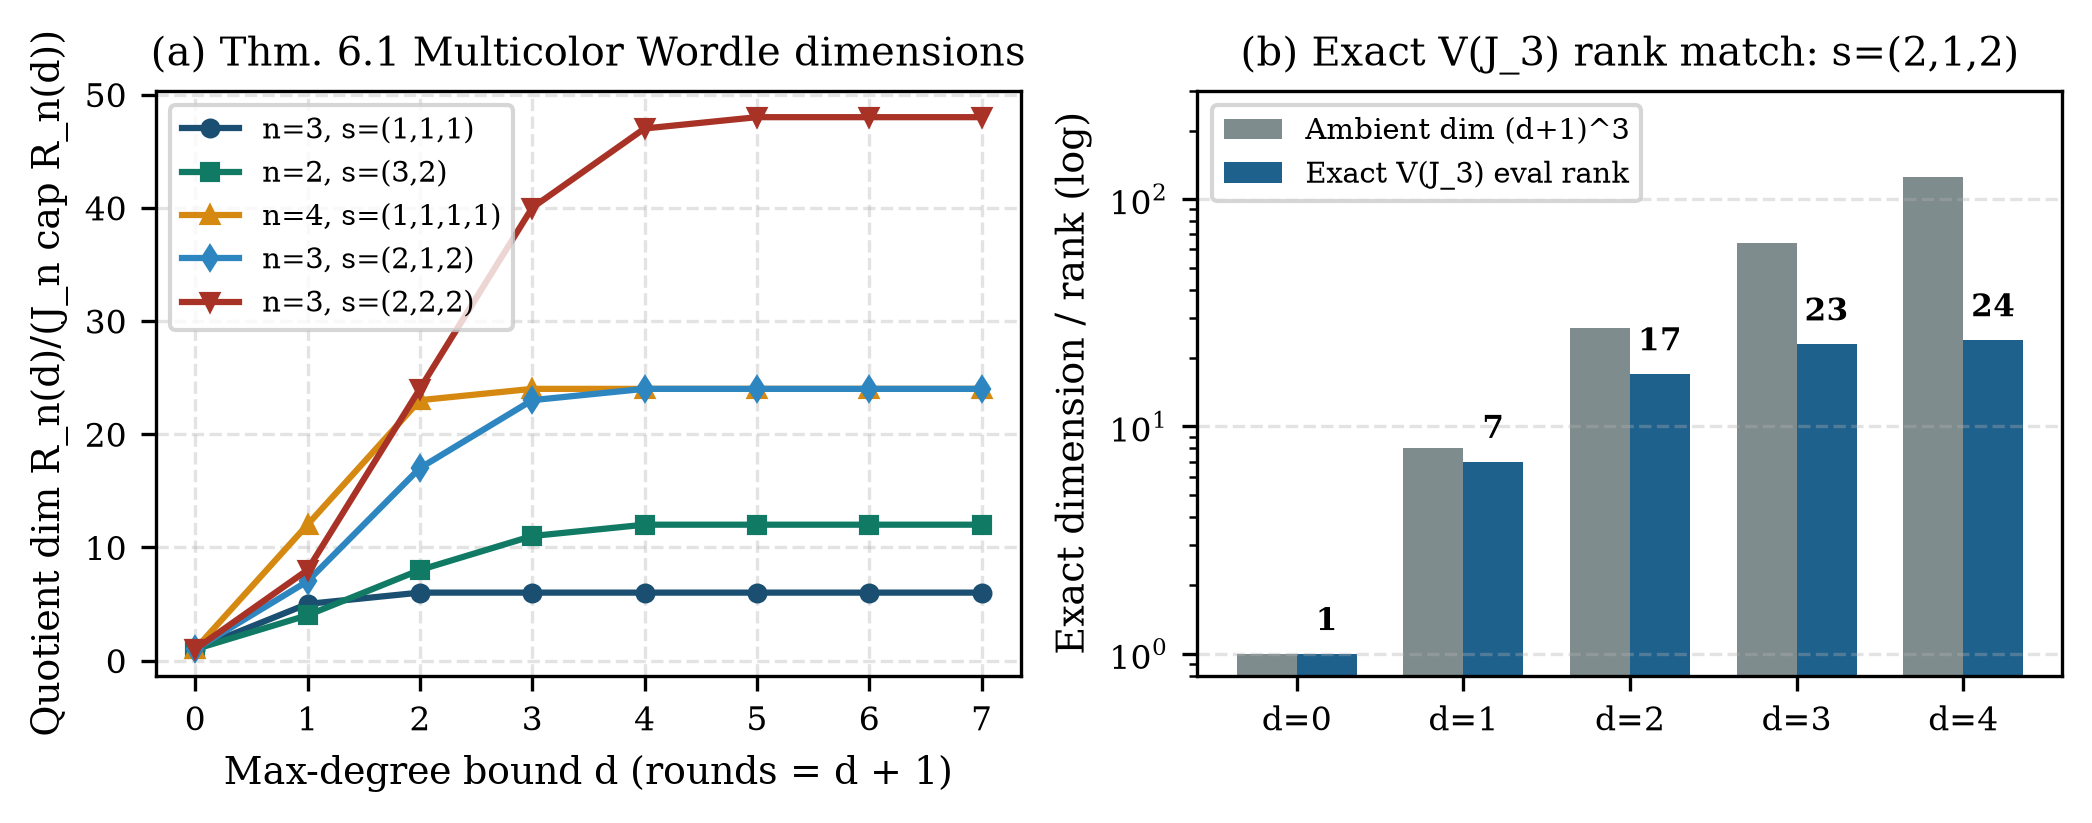
\includegraphics[width=\columnwidth]{figures/fig1_wordle_dims_and_eval_rank.png}
\caption{(a)~Exact Theorem~6.1 cumulative quotient dimensions across five Multicolor Permutation Wordle configurations. (b)~Ambient monomial dimension $(d+1)^3$ versus exact $V(J_3)$ rational evaluation rank for $s=(2,1,2)$ ($d=0..4$).}
\label{fig:dims-eval}
\end{figure}

\paragraph{2. Gap-free strictness defect grid and exact Koszul complexes.}
Figure~\ref{fig:grid-koszul}(a) maps the exact strictness defect $(\dim R_2(b) - \mathrm{rank}\,\delta_1) - \mathrm{rank}\,E_{V(J_2)}(R_2(b))$ across all 16 multidegrees $b \in [0..3]^2$ for $N=M=2, s=(1,1)$: defect is $0$ across all 10 gap-free points ($|b_1-b_2| \le 1$) and jumps to $1$ at $(0,2),(2,0)$ and $2$ at $(0,3),(3,0)$, visually confirming Remark~A.1. Figure~\ref{fig:grid-koszul}(b) compares $F_0^b$, $F_1^b$, and exact quotient dimensions across our four Mode~1 Koszul complexes.

\begin{figure}[t]
\centering
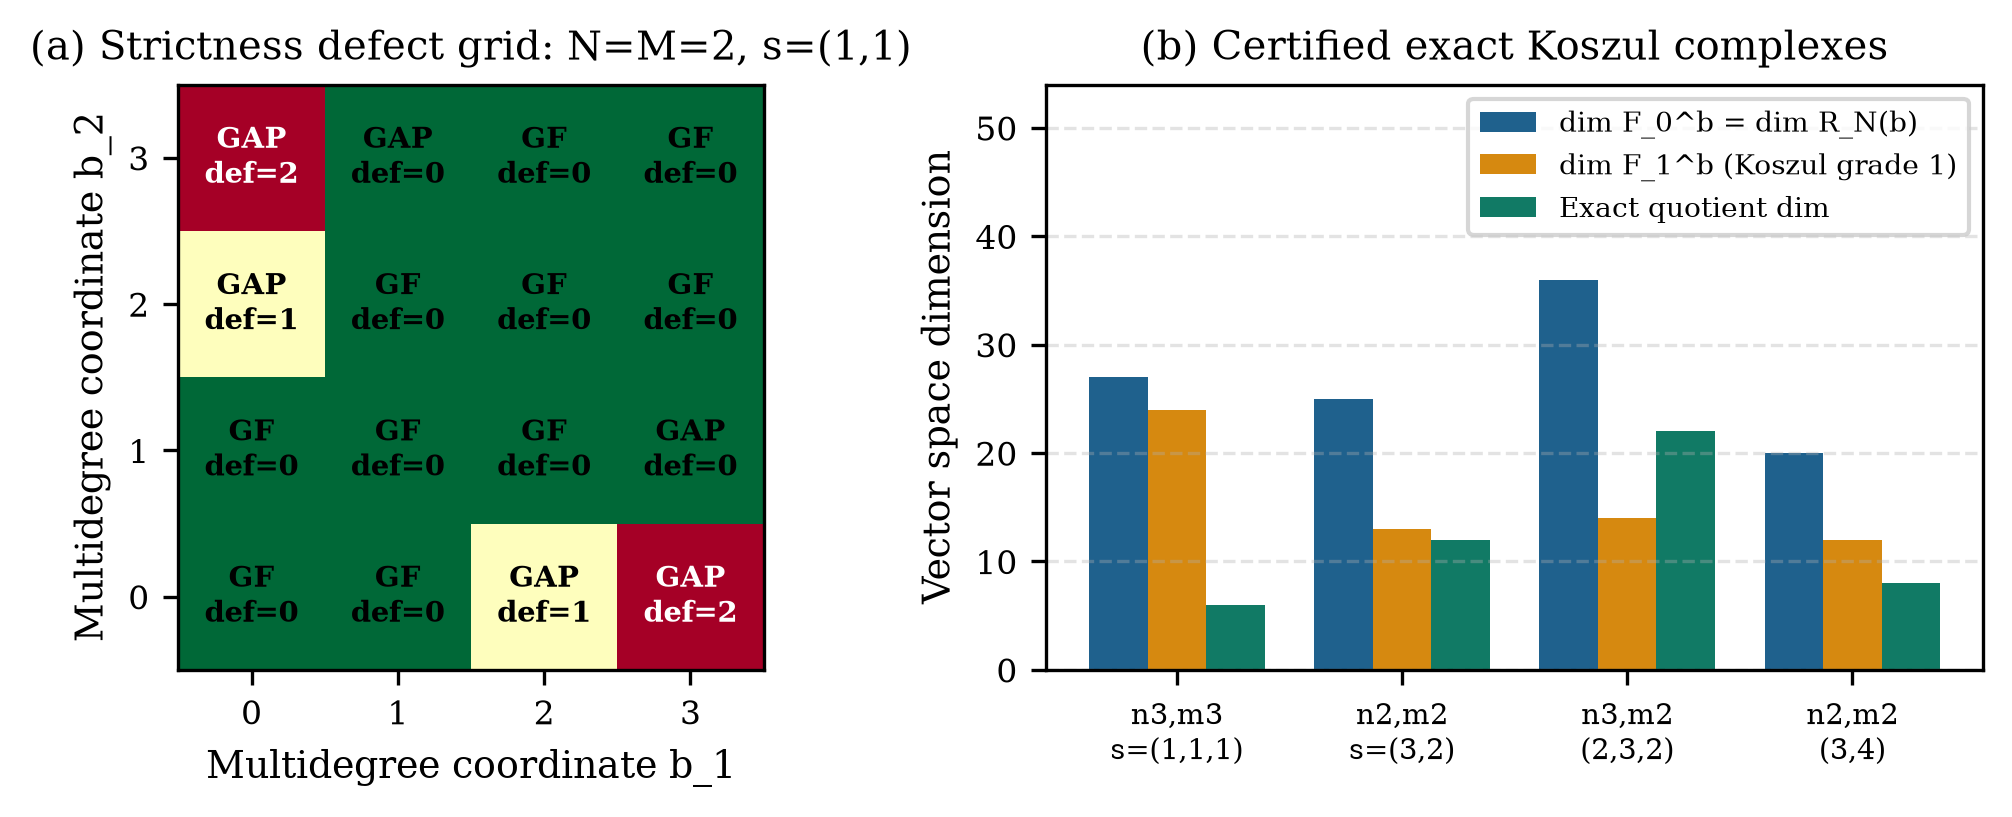
\includegraphics[width=\columnwidth]{figures/fig2_strictness_grid_and_koszul.png}
\caption{(a)~Exact strictness defect across $b \in [0..3]^2$ for $N=M=2, s=(1,1)$: zero on every gap-free point, strictly positive at $(0,2),(2,0),(0,3),(3,0)$. (b)~Certified grade dimensions and quotient dimensions across all four Mode~1 Koszul complexes.}
\label{fig:grid-koszul}
\end{figure}

\paragraph{3. 16-certificate atlas and 57-attack red-team suite.}
Table~\ref{tab:atlas} and Figure~\ref{fig:atlas} summarize all 16 canonical certificates, replayed with zero floats in $0.050$--$66.09\,\mathrm{ms}$ (largest matrix: $48\times 64$ exact rational evaluation on $V(J_3)$ for $s=(2,2,2), d=3$, rank $40$). In \texttt{tests/test\_suite.py}, exhaustive grid and $V(J_3)$ rank cross-checks and 57/57 live adversarial forgeries (non-gap-free Mode~1 inputs, gap-free Mode~3 fakes, invalid $w \notin \ker\delta_1^T$, $s_k=3$ in Mode~4, wrong ranks/Euler characteristics) are rejected with \texttt{KoszulWordleCertificateError}.

\begin{figure}[t]
\centering
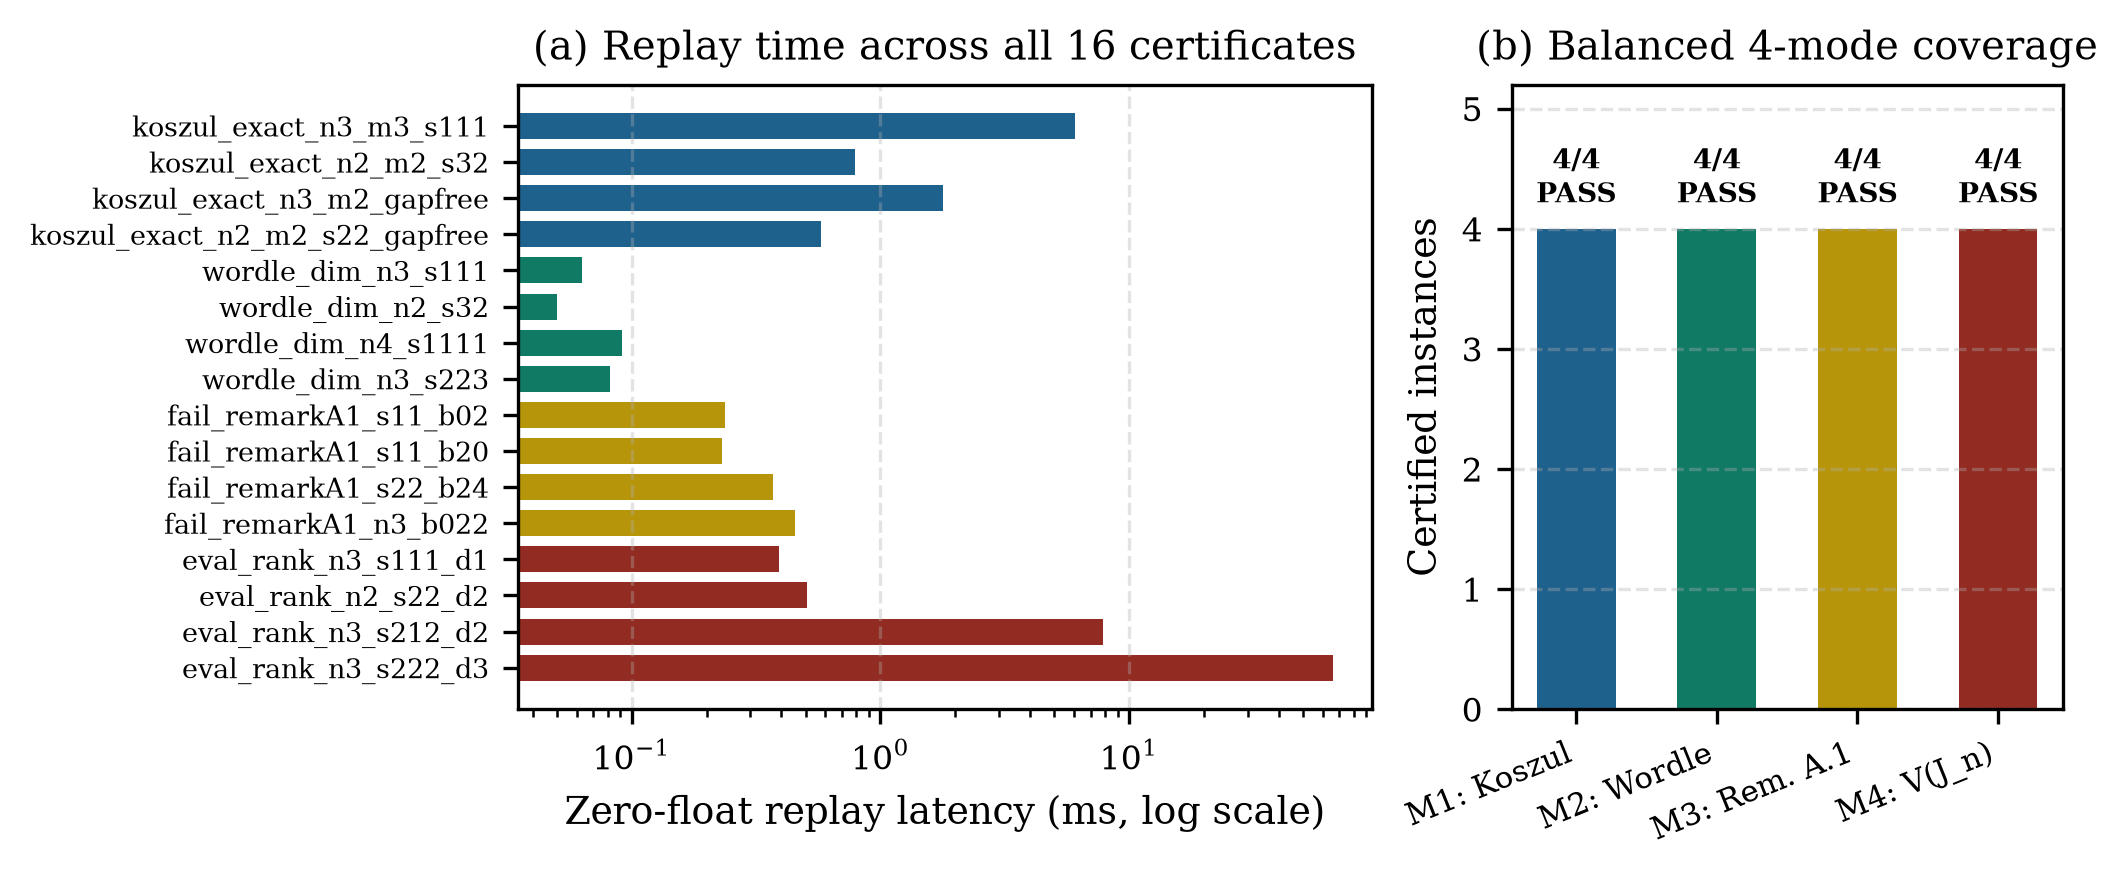
\includegraphics[width=\columnwidth]{figures/fig3_atlas_summary.png}
\caption{(a)~Zero-float replay latency across all 16 canonical \texttt{KOSZUL-WORDLE-CERT-1.0} certificates ($0.050$--$66.09\,\mathrm{ms}$, log scale). (b)~Balanced 4-per-mode coverage across all four verification modes.}
\label{fig:atlas}
\end{figure}

\begin{table}[t]
\centering
\caption{Summary of all 16 exact-$\QQ$ \texttt{KOSZUL-WORDLE-CERT-1.0} certificates (zero floating-point arithmetic; reference-machine replay latency in ms).}
\label{tab:atlas}
\resizebox{\columnwidth}{!}{%
\begin{tabular}{@{}lllr@{}}
\toprule
Certificate File (stem) & Mode & Key Exact Witness & ms \\
\midrule
\texttt{koszul\_exact\_n3\_m3\_s111} & M1 & $b=(2,2,2)$, dims $[27,24,3,0] \to 6$ & 6.059 \\
\texttt{koszul\_exact\_n2\_m2\_s32} & M1 & $b=(4,4)$, dims $[25,13,0] \to 12$ & 0.793 \\
\texttt{koszul\_exact\_n3\_m2\_gapfree} & M1 & $b=(2,3,2)$, dims $[36,14,0] \to 22$ & 1.778 \\
\texttt{koszul\_exact\_n2\_m2\_s22\_gapfree} & M1 & $b=(3,4)$, dims $[20,12,0] \to 8$ & 0.579 \\
\texttt{wordle\_dim\_n3\_s111} & M2 & $s=(1,1,1)$: $d_{\max}=2$, $6$ perms & 0.063 \\
\texttt{wordle\_dim\_n2\_s32} & M2 & $s=(3,2)$: $d_{\max}=4$, $12$ perms & 0.050 \\
\texttt{wordle\_dim\_n4\_s1111} & M2 & $s=(1^4)$: $d_{\max}=3$, $24$ perms & 0.091 \\
\texttt{wordle\_dim\_n3\_s223} & M2 & $s=(2,2,3)$: $d_{\max}=6$, $72$ perms & 0.082 \\
\texttt{fail\_remarkA1\_s11\_b02} & M3 & $b=(0,2)$: $w^T\delta_1=0, w^T Z=2$ & 0.238 \\
\texttt{fail\_remarkA1\_s11\_b20} & M3 & $b=(2,0)$: $w^T\delta_1=0, w^T Z=6$ & 0.231 \\
\texttt{fail\_remarkA1\_s22\_b24} & M3 & $b=(2,4)$: $w^T\delta_1=0, w^T Z=12$ & 0.370 \\
\texttt{fail\_remarkA1\_n3\_b022} & M3 & $b=(0,2,2)$: $w^T\delta_1=0, w^T Z=4$ & 0.455 \\
\texttt{eval\_rank\_n3\_s111\_d1} & M4 & $|V|=6$, $d=1$: rank $=5$ & 0.390 \\
\texttt{eval\_rank\_n2\_s22\_d2} & M4 & $|V|=8$, $d=2$: rank $=7$ & 0.505 \\
\texttt{eval\_rank\_n3\_s212\_d2} & M4 & $|V|=24$, $d=2$: rank $=17$ & 7.838 \\
\texttt{eval\_rank\_n3\_s222\_d3} & M4 & $|V|=48$, $d=3$: rank $=40$ & 66.087 \\
\bottomrule
\end{tabular}}
\end{table}

\section{Scope, Limitations, and Conclusion}\label{sec:conclusion}
This work machine-checks the finite Koszul-complex differential, inductive Euler-characteristic telescoping, Multicolor Permutation Wordle generating-function counts, Appendix~A Remark~A.1 gap-free counterexamples, and exact rational zero-set evaluation ranks of Smithline~\cite{smithline2026koszul}. It does \emph{not} formalize the general-$(N,M)$ mapping-cone induction (Theorem~5.1) or game-theoretic strategy reduction (Theorem~1.1) in Lean~4. Within its verified scope, the Lean~4 kernel and \texttt{KOSZUL-WORDLE-CERT-1.0} auditor deliver exact, manifest-locked verification for filtered Koszul resolutions and Multicolor Wordle dimension bounds.

\bibliographystyle{plain}
\bibliography{references}
\end{document}
